% IEEE Paper Template for A4 Page Size
% Sample Conference Paper using IEEE LaTeX style file for A4 page size.
% Copyright (C) 2006-2008 Causal Productions Pty Ltd.
% Permission is granted to distribute and revise this file provided that
% this header remains intact.
% 
% REVISION HISTORY
% 20080211 changed some space characters in the title-author block
%
\documentclass[10pt,conference,a4paper]{IEEEtran}
\usepackage{times,amsmath,amssymb,epsfig}
\usepackage{epstopdf}

%
%%%%%%%%%%%%%%%%%%%%%%%%%%%%%%%%%%%%%%%%%%%%%%%%%%%%%%%%%%%%%%%%%%%%%%%%%%%%%%%%
%%%%%%%% USER DEFINED PACKAGES:
\usepackage[utf8]{inputenc} 
\usepackage[T1]{fontenc}     
\usepackage[english]{babel}


%\usepackage{bookman}
%\usepackage{charter}
%\usepackage{newcent}
%\usepackage{lmodern}
%\usepackage{mathpazo}
%\usepackage{mathptmx}
%\usepackage{cm}

\usepackage{booktabs}% http://ctan.org/pkg/booktabs
\usepackage{tabularx}% http://ctan.org/pkg/tabularx
\usepackage{makecell}
\usepackage{array}
\usepackage{multirow}
\usepackage{layout}  
\usepackage{color}
\usepackage{colortbl}
\definecolor{red1}{RGB}{240,40,40}
\definecolor{grn1}{RGB}{40,240,40}
\definecolor{blu1}{RGB}{40,40,240}
\definecolor{vraipos}{rgb}{0.04,0.2,0.04}
\definecolor{vraineg}{rgb}{1,1,1}
\definecolor{fauxpos}{rgb}{1,0.8,0.8}
\definecolor{fauxneg}{rgb}{0.1,0.6,0.1}
\usepackage[top=2cm, bottom=2cm, left=2cm, right=2cm]{geometry}
\usepackage{url}

\hyphenation{DPLoS}
\graphicspath{{./images/}}

\usepackage[breaklinks=true,bookmarks=false]{hyperref}
%%%%%%%%%%%%%%%%%%%%%%%%%%%%%%%%%%%%%%%%%%%%%%%%%%%%%%%%%%%%%%%%%%%%%%%%%%%%%%%%

\title{Building a Crowdsourcing based Disabled Pedestrian Level of Service application using Computer Vision and Machine Learning}
%
\author{%
\,Anonymous VCIP Submission\\
\,Paper ID:

\iffalse
% author names are typeset in 11pt, which is the default size in the author block
% {First Author{\small $~^{\#1}$}, Second Author{\small $~^{*2}$}, Third Author{\small $~^{\#3}$},
% Removed for anonymous submission
{Nicolas Blanc{\small $~^{\#1}$}, Zhan Liu{\small $~^{*5}$}, Jens Ingensand{\small $~^{\#2}$}, Romain Sandoz{\small $~^{\#3}$},}
\,\\
{Olivier Ertz{\small $~^{\#4}$}, Jean-Christophe Loubier{\small $~^{*6}$}, Diego Rojas{\small $~^{*7}$},
Sokhn Maria{\small $~^{*8}$} }
{}

% add some space between author names and affils
\vspace{1.6mm}\\
\fontsize{10}{10}\selectfont\itshape
% 20080211 CAUSAL PRODUCTIONS
% separate superscript on following line from affiliation using narrow space
% $^{\#}$\,First-Third Department, First-Third University\\ %  Removed for anonymous submission
% Address Including Country Name\\ %  Removed for anonymous submission

$^{\#}$\,{University of Applied Sciences Western Switzerland,}\\
{School of Management and Engineering Vaud,}\\
{Rte de Cheseaux 1,} \\
{CH-1400 Yverdon-les-Bains}
\,\\
\\
$^{*}$\,{University of Applied Sciences Western Switzerland,}\\
{School of Management \& Tourism,}\\
{Rte de la Plaine 2, PO box 80, }\\
{CH-3960 Sierre}
\,\\ 
\\
\fontsize{9}{9}\selectfont\ttfamily\upshape
%
% 20080211 CAUSAL PRODUCTIONS
% in the following email addresses, separate the superscript from the email address
% using a narrow space \,
% the reason is that Acrobat Reader has an option to auto-detect urls and email
% addresses, and make them 'hot'.  Without a narrow space, the superscript is included
% in the email address and corrupts it.
% Also, removed ~ from pre-superscript since it does not seem to serve any purpose
% $^{1}$\,first.author@first-third.edu\\ % Removed for anonymous submission
% $^{3}$\,third.author@first-third.edu %  Removed for anonymous submission
$^{1-4}$\,\{nicolas.blanc1,
jens.ingensand,
romain.sandoz,
olivier.ertz\}@heig-vd.ch\\ % Removed for anonymous submission
$^{5-7}$\,\{zhan.liu,
jchristophe.loubier,
diego.rojas,
maria.sokhn\}@hevs.ch %  Removed for anonymous submission

\,\\ 
\\

% add some space between email and affil
\vspace{1.2mm}\\
\fontsize{10}{10}\selectfont\rmfamily\itshape
% 20080211 CAUSAL PRODUCTIONS
% separated superscript on following line from affiliation using narrow space \,
% $^{*}$\,Second Company\\ %  Removed for anonymous submission
% Address Including Country Name\\ %  Removed for anonymous submission
\,\\ 
\\

\fontsize{9}{9}\selectfont\ttfamily\upshape
% 20080211 CAUSAL PRODUCTIONS
% removed ~ from pre-superscript since it does not seem to serve any purpose
%$^{2}$\,second.author@second.com %  Removed for anonymous submission
\,
\fi
} % end of author

%
%%%%%%%%%%%%%%%%%%%%%%%%%%%%%%%%%%%%%%%%%%%%%%%%%%%%%%%%%%%%%%%%%%%%%%%%%%%%%%%%
\begin{document}
%%%%%%%%%%%%%%%%%%%%%%%%%%%%%%%%%%%%%%%%%%%%%%%%%%%%%%%%%%%%%%%%%%%%%%%%%%%%%%%%
\maketitle

% INCLUDES COPYRIGHT NOTICE: one of three copyright notice should be included. Uncomment the appropriate line below, according to the authors affiliation:
\begin{figure}[b]
\parbox{\hsize}{\em
%information about the event:
%IEEE VCIP'14, Dec. 7 - Dec. 10, 2014, Valletta, Malta.

%copyright notice: one of three copyright notices below should be included. Uncomment the appropriate line, according to the authors affiliation:
%000-0-0000-0000-0/00/\$31.00 \ \copyright 2014 IEEE.
%U.S. Government work not protected by U.S. copyright.
%???-?-????-????-?/10/\$??.?? \copyright 2014 Crown.
}\end{figure}


\begin{abstract}
   Availability of global and scalable tools to assess disabled pedestrian level of service (DPLoS) is a real need but still a challenge in today’s world. It is usually summarized by lacking of tools that can ease the measurement of a level of service adapted to disabled people, and the limitation concerns the availability of information regarding the existing level of service in real time as well. This paper aims to use advanced computer vision technologies and benefits from the prevalence of handheld devices in order to respond to those needs. Our approach allows the development of a navigation tool with crowdsourcing technologies that can help a disabled person to move around a city, and suggest the most adapted routes according to the person’s disabilities. This solution provides the opportunity to get the up-to-date data with valuable field observations.
\\[1\baselineskip]
\end{abstract}


% NOTE keywords are not used for conference papers so do not populate them
\iffalse
\begin{keywords}
crowdsourcing, computer vision, mapping application, disable pedestrian level of service
\end{keywords}
\fi
%

%################################################################################
%################################################################################
\section{Introduction}
%################################################################################
%################################################################################

Creating the disabled pedestrian map-based routing is a challenge for both researchers and practitioners. Disabled pedestrian level of service (DPLoS) have been studied and discussed by more and more people. One of the most important reason is maps-based routing solution provides information about the available facilities of transitory obstacles to enable people with mobility disabilities to travel more easily. In fact, the demand for disabled pedestrian level of services is enormous. According to World Health Organization \cite{who2017}, over a billion people live with some form of disability. This correspond to about 15\% of the world’s population, and between 110 and 190 million adults have very significant difficulties in functions that include the wheelchair users. The interdisciplinary researches are working together to make contributions in this domain.

Despite the existence of standards and regulations to increase the ability of both disabled people and persons with limited mobility to independently use pedestrian networks, there is still a lack in replicable, objective, cost-effective systems to assess pedestrian infrastructure \cite{frackelton2013measuring}. Therefore, two main limitations have been identified. On one hand, there is a lack of tools that can ease the measurement of a level of service (LoS) adapted to disabled people. These tools can help assess the level of accessibility of a pedestrian network. On the other hand, the missing of the availability of information regarding the existing level of service in real time causes problems. When moving through a network, a disabled person needs this kind of information to take a right decision.

In this study, we present a technical approach, named CrowDPLoS, which uses advanced computer vision technologies and benefits from the prevalence of handheld devices in order to meet the challenges discussed above. This approach allows the development of a navigation tool with crowdsourcing technologies that can help people with disabilities to move around a city suggesting the most adapted routes according to the person’s disabilities. To summarize, the best route in our approach is based on the highest level of service of route and adapted to the user’s handicap. Specifically, we give people with mobility impairments, mainly wheelchair users, a mean to travel safely and with ease through a modern urban area by applying the algorithms of computer vision. These algorithms use crowdsourced images taken by the users of a mobile application in order to determine a level of service adapted to disabled pedestrians.

This paper is organized as follows: section 2 presents a summary of the related works of computer vision based techniques and crowdsourcing in disabled pedestrian level of service. In section 3, we explain our approaches to develop models that measure a crowdsourcing based disabled pedestrian level of service for pedestrian networks, which are applied the technologies of computer vision and machine learning. Finally, we conclude with a summary of the current work, and we present suggestions for future research.



%################################################################################
%################################################################################
\section{Related work}
%################################################################################
%################################################################################
%This section will present the related work in the fields of each working packages.

%################################################################################
\subsection{Models of disabled pedestrian level of service}
%################################################################################

%Level of Service (LoS) has long been studied for pedestrian (PLoS) \cite{landis_modeling_2001, gallin_quantifying_2001}. The former proposed a model that can help crossroads design and prioritize the needs for local governments. 

Safety and accessibility of pedestrian infrastructure regulation developments have historically been supported by governmental institutions. For example in the United States was carried out the Americans with Disabilities Act (ADA) in 1990. The ADA was designed in order to guide the implementation of regulations and specifications for pedestrians.
 
The first formalization of sidewalks performance assessments was carried out by \cite{fruin1971pedestrian}. His approach is the only quantifying established methodology to measure the capacity of sidewalks \cite{landis_modeling_2001}. The practical usage of his methodology has its limitations, in fact only around 3 percent of the sidewalks could be effectively assessed by Fruin’s method. 

Given that sidewalks are one of the most important and secure places for pedestrian to walk on in urban areas, several studies have focused their researches on characterizing and assessing sidewalks accessibility, even based on perceived security from the pedestrian point of view \cite{tan_research_2007}. According to Landis et al. \cite{landis_modeling_2001}, it is more difficult to assess walking conditions than assessing vehicular roadways.  Furthermore research focused on PLoS for disabled people (DPLoS) is rather new. Asadi et~al. \cite{asadi-shekari_zohreh_disabled_2013} have for example calculated 10 main feature indicators based on several studies and guidelines regarding the presence of facilities for disabled people, like wheelchair users or blind people. Once the 10 DPLoS indicators were developed they proceeded to establish 10 PLoS indicators with the same methodology.  The combination of the DPLoS and PLoS is a General Pedestrian Level of Service (GPLoS), which assesses the inclusive walking conditions for both pedestrians and disabled users. Readers interested in a more exhaustive literature review on the development of PLoS are referred to Asadi et~al.
 
%################################################################################
\subsection{Computer Vision and machines learning based techniques for assessing relevant street features}
%################################################################################
Historically, computer vision tends to extract the most important features from images like color histograms, edges \cite{canny_computational_1986} or specific patterns. %\cite{duda_use_1972}.
%Segmentation by watershed algorithms \cite{meyer_morphological_1990, beucher_segmentation:_1993} using graph-based techniques \cite{felzenszwalb_efficient_2004} or oriented gradient \cite{malisiewicz_ensemble_2011} gives the ability to well enough isolate regions on an image.
Hough transform is a well know line detector that may be used to extract street borders %\cite{illingworth_survey_1988,ballard_generalizing_1981,kiryati_probabilistic_1991} 
\cite{kiryati_probabilistic_1991} 
as well as vanishing point extraction. %\cite{se_road_2003,wang2004lane,kong2009vanishing}.
%\cite{wang2004lane,kong2009vanishing}.
%\cite{kong2009vanishing}. %The latter relies on image geometric properties %\cite{forsyth2002computer,hartley2003multiple,szeliski2010computer}.
%\cite{szeliski2010computer}.


%Sky views are also known to provide good enough classification results, especially for crosswalks detection \cite{berriel_deep_2017}.
The slope of a street and the detection of obstacles are focus of research in the subject of accessibilities. The using of geolocation with odometric data, mainly GPS trajectory, is a common solution. Hara et~al. \cite{hara_tohme:_2014} show how computer vision may be used to determine accessibility from physical features of the real world based on Google Street View images coupled with machine learning techniques. Within the latter domain, convolutional neural networks (CNN) are especially designed to extract features from images \cite{lecun1995convolutional}. 
Based on these techniques, field of autonomous driving also brings a solid background for street images segmentation \cite{alvarez2012road}. Existing street scene datasets %like Cityscapes %\cite{Cordts_2016_CVPR} or Mapillary
along with semantic segmentation and region-based methods \cite{neuhold2017mapillary} have proven the need of fine grained labeled images to suit a particular task. Using weights of low level features extracted by some CNN on these datasets may be a good starting point to build a more specific architecture dedicated to the DPLoS features extraction.


Moreover, steroscopic vision %\cite{szeliski2010computer} 
provides at low cost the useful depth information as a disparity map. This is done by computing a 3D point cloud from stereo images pairs, which can help to better isolate relevant objects.
Coughlan and Shen \cite{coughlan_terrain_2007} %and Ivanchenko et~al. \cite{ivanchenko_computer_2008} %\cite{zbontar2016stereo} 
make use of an embeded stereo camera to detect negative obstacles on the wheelchair user's path. 
% Embedded based techniques make use of a camera to detect crosswalk  \cite{ivanchenko_crosswatch:_2008} 
%or straight paths using stereoscopic based vision \cite{asad_smartphone_2012}. 
%Active scanning devices directly provide additional data of the environment. 

%\cite{smith_classification_2013} used a more global approach coupled with a random forest classifier to identify sidewalks on street view images.

% \cite{association_for_computing_machinery_acm_tohme:_nodate} % yt









But there are still two main bottlenecks to build a supervised computer vision classifier based on machine learning. These are 1) data acquisition and 2) the presence of high quality associated labels. If nowadays huge amount of data is available, they may not be well enough labeled nor suited to a given specific task, hence well managed crowdsourcing tasks may provide an invaluable help in both.

%################################################################################
%\subsection{Image detection Using Machine Learning algorithms}
%################################################################################


%################################################################################
\subsection{Crowdsourcing in disabled pedestrian level of service}
%################################################################################
Research on disabled pedestrian level of service (DPLoS) is relatively new. The analytical methods to estimate the DPLoS is not only considered as a narrow range of pedestrians, but also need to apply more diverse pedestrian populations with different characteristics, to ensure inclusive walking conditions. Therefore, a good quality of crowdsourced data from citizens is the key element to create the DPLoS. Liu et al. \cite{liu2018} identified three useful techniques for improving crowdsourced data quality when building accessibility maps, including qualification tests, reputation system, and aggregation techniques. Their findings highlighted that the accuracy rate has a significant increase after applying the intervention of quality control methods. Moreover, \cite{brovelli_webbased_2014} and \cite{minghini_multi-dimensional_2014} shown how participatory Geographic Information System (GIS) using Free and Open Source Software (FOSS) may help provide high quality open-GIS data and make them available to the public using web technologies. 

%mostafavi2015mobilisig
Other studies \cite{comai_mapping_2015, gharebaghi2017confidence} focused on mapping the level of accessibility of street networks %(MEP: Map for Easy Paths)
using an end-user design approach, while
%A 2015 interdisciplinary urban data science program of the University of Washington \cite{rokem_building_2015} has seen 2 projects related to impaired people mobility. One of them, called 
the OpenSideWalk project also
\cite{noauthor_opensidewalks_nodate} 
%\cite{noauthor_opensidewalks_nodate,bolten_urban_2015,tanweer_mapping_2017} 
investigate routing techniques for sidewalk graph analysis in order to propose the better paths for disabled people. The latter is now proposing a schema to better and more finely represents sidewalks as separate footways from the drivable roads in OpenStreetMap (OSM).%\footnote{\url{https://www.opensidewalks.com/}} \cite{noauthor_opensidewalks_nodate}.

%Even the tourism industry may take some advantages of disabled accessibility researches \cite{israeli_preliminary_2002}.

%In Switzerland, one can easily find some architectural guidelines related to disabled pedestrians \cite{schmidt_directives_2003} mainly based on Swiss Standard (SN).


In this study, we follow the guidelines from literatures and apply selective recruitment and training of participants to provide the high-quality crowdsourcing data in addition to computer vision based techniques.

%################################################################################
\subsection{Combination of crowdsourcing and computer vision to evaluate the DPLoS model}
%\subsection{Coupling the two techniques (reuse in CV or ML, or delete it)}
%################################################################################
Computer vision is an useful technology for the autonomous driving and objects detection, but features extraction relies frequently on domain experts. Integrating crowdsourcing is not an easy task. A recent survey by Kovashka et~al. \cite{kovashka2016crowdsourcing} addressed some of the most important questions regarding computer vision and crowdsourcing, which provided useful general guidelines. But only a few studies took advantages of both techniques for DPLoS assessment and the application design.
Hara and Froehlich \cite{hara_feasibility_2012}
have shown the opportunity of integrating final users in the design of an application devoted to disabled pedestrian and to assess scaled street segments aptitude.

%\cite{hara_scalable_2014, hara_characterizing_2015}
%More recently, they have shown how to combine crowdsourcing and computer vision on Google Street View images to collect informations on disabled pedestrians accessibility \cite{hara_characterizing_2015}. 
More recently, Hara et~al. \cite{hara_tohme:_2014,hara_characterizing_2015} designed a specific tool which makes use of Amazon Mechanical Turk (AMT) to achieve rapidly with lower costs on images detection tasks. Recall of AMT workers combined with computer vision algorithms was higher and faster than AMT workers alone. Therefore, combination of both technologies could provide a better accuracy on objects detection. The challenges of this kind of approach are reflected in how to motivate the participants for data acquisition and how to ensure the quality of collected data. The latter requires substantial time a or money investments and high knowledge demanding operations.
%\cite{hara_combining_2013, hara_improving_2013, hara_improving_2015}. 
%\cite{hara_improving_2015}. 
%Thus, computer vision, especially when combined with machine learning, endorse an important role in detecting features.

%\cite{von_ahn_labeling_2004,von2006peekaboom}.

%################################################################################
%\subsection{Graph and network analysis}
%################################################################################
%\cite{boeing_osmnx:_2017}
%\cite{bolten_urban_2015}




%################################################################################
%################################################################################
\section{Methodology and preliminary results}
%################################################################################
%################################################################################
Based on the relevant literature, our research methodology is divided into three main phases: 1) the creation of the DPLoS model; 2) the establishment of a pedestrian network at a city-scale level; and 3) the design of a computer vision and machine learning architecture dedicated to features detections, coupled with crowdsourcing applications to collect data, digitize and label features and evaluate the detection results.

%################################################################################
\subsection{\colorbox{yellow}{DPLoS model}}
%################################################################################
\colorbox{red}{Jean-Christophe Loubier}

.........


The DPLoS established model retains the 4 following features based on literature guidelines plus a: % set ranges here
\begin{itemize}
\item slope
\item sidewalks width and presence of obstacles
\item crosswalks and security signals (e.g. pedestrian light, refuge island)
\item presence of curb ramps to cross the road
\item coating quality (e.g. pavement, smooth concreet)
\end{itemize}

A normalized score $S_{i}$ for each feature $i$ is then weighted to compute a global DPLoS score for any street edge as eq.\,\ref{dplos1} shows.
\begin{equation}
\frac{1}{5}\sum\limits_{i=1}^5 S_{i}\cdot{}w_{i}
\label{dplos1}
\end{equation}
Weights $w_{i}$ have to be determined based on local conditions and street users perception.
%################################################################################
\subsection{Pedestrian graph as an input}
%################################################################################
DPLoS computation for street edges requires a pedestrian graph as an input.
In order to build this graph, we relied on existing open data such as National Map Agency (NMA) Cadastral Survey, OSM streets and footways. In order to obtain the high quality vector data to draw the pedestrian graph, we used the high resolution satellite data to extract a road network with segmentation-based classification methods.

\iffalse
\begin{itemize}\setlength\itemsep{0.0em}
\item National Map Agency (NMA) Cadastral Survey,
\item NMA vector data, if available or
%\item the Topographic Landscape Model (TLM) of the Federal Office of Topology, swisstopo,
\item OSM streets and footways
%\item any third party road network.
\end{itemize}
\fi

The figure \ref{pedestriangraph} illustrated the results to show a pedestrian network by applying the data from OpenStreetMap. This graph was created by using is a dedicated tool named OSMnx \cite{boeing_osmnx:_2017}. The light lines display the available sidewalks information on this network. 

\begin{figure}[ht]
\begin{center}
%\fbox{\rule{0pt}{2in} \rule{0.9\linewidth}{0pt}}
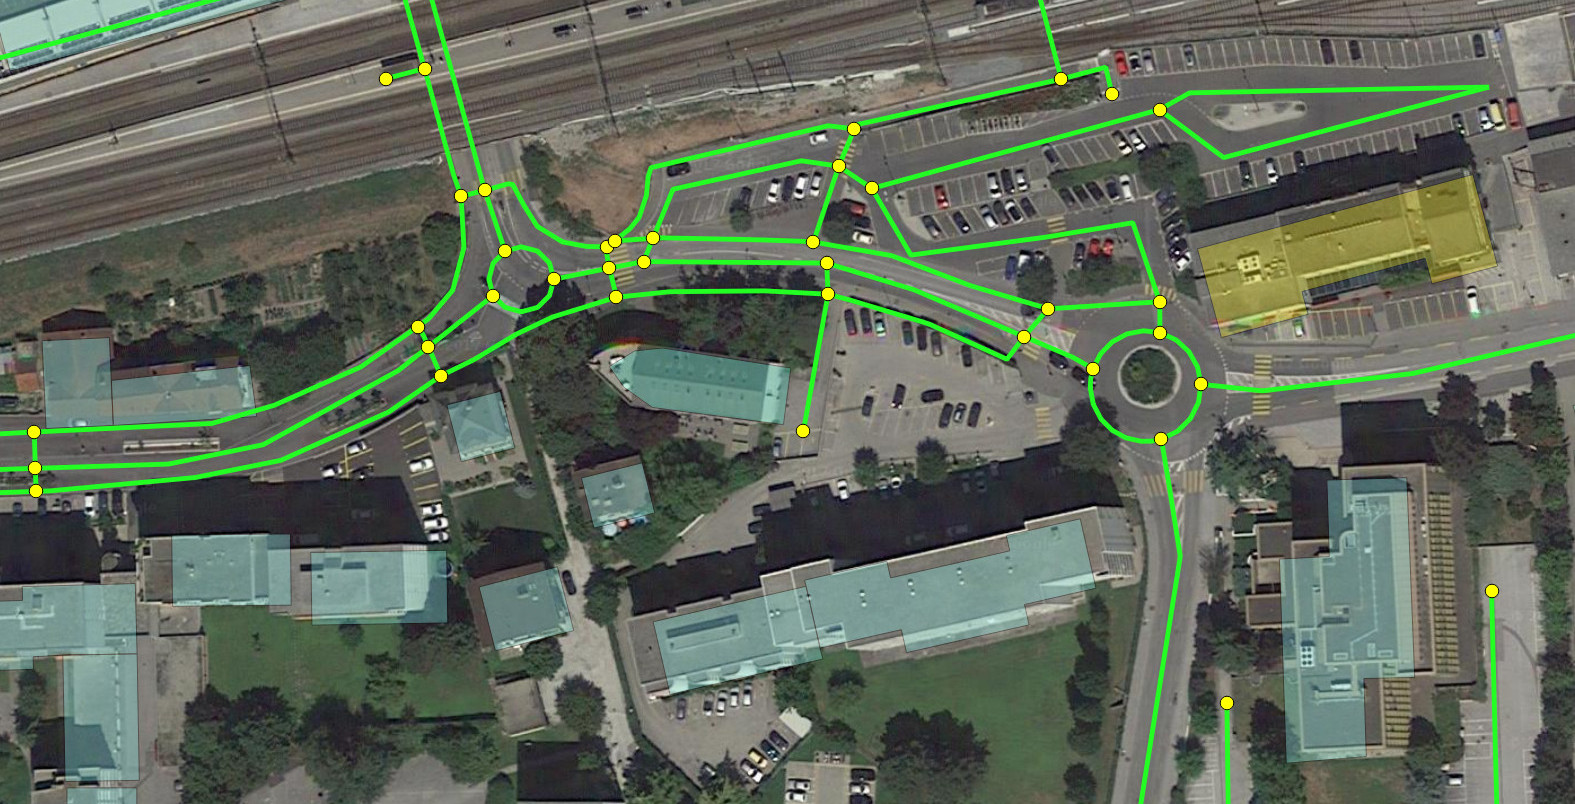
\includegraphics[width=1.0\linewidth]{OSM_walk_graph_022.jpg}
\end{center}
   \caption{Part of the pedestrian network extracted from OpenStreetMap (OSM) data (light) in a downtown area.}\label{pedestriangraph}
\end{figure}


%################################################################################
\subsection{Combination of algorithms and crowdsourcing}
%################################################################################
%The development of an application, %even if located at later stage in the global process, 
%should be included as soon as possible. 

In this section, we use four steps to explain how the computer vision algorithms and crowdsourcing technologies could be combined together. These steps contain: 1) footways network update; 2) data acquisition; 3) images features digitizing and labeling; and 4) end-user route choice and update abilities. Each of these steps will need the development of a specialized application or tool.


%#####################################
\subsubsection*{1) Footways network update}
%#####################################
The initial pedestrian network  may not be totally fulfilled (fig.\,\ref{pedestriangraph}) due to its voluntary basis and interest of local citizen for geographic data \colorbox{green}{<- why not be fulfilled}. A first tool \colorbox{yellow}{which tool? existing tool or our developed tool? } 
\colorbox{green}{=>explained above, lines 1-2 of this column}
\colorbox{yellow}{Can you describe it with the functions? How this tool can help to make more precision?}
\colorbox{green}{=>here under:, it's the use of a recent orthophoto, like google satellite imagery with 30cm resolution that make it possible}
will be developed to give crowd-workers a pleasant way to complete or make it fit the actual reality more precisely based on a recent orthophoto background with a 30\,cm minimal resolution and a sub-meter accuracy. %This part may be desktop-oriented for a more comfortable data entry.


%#####################################
\subsubsection*{2) Data acquisition and geolocation}
%#####################################
A second application \colorbox{yellow}{second step? what is the first application?}\colorbox{green}{the first tool is: 1) Footways network update, as line 1-2 of this columns explains it}, % which may be mobile-oriented 
would serve as a feeding source for raw images. 

Everyone can take a picture with a handheld mobile device. An upload tool linked to a spatial database will be build to collect users' photographs.\colorbox{yellow}{which database?} Along with existing street pictures sources like Google Street View %\cite{sweden_street-level_nodate,} \footnote{\url{https://www.mapillary.com/}} \cite{sweden_street-level_nodate},
these images will be used as raw data input for the digitizing stage.
If position and orientation (azimuth) values are know from a GPS and compass, they are stored along the picture. Otherwise, a geolocation tool will proposed to the user to geolocate and orient its photograph before uploading it. %A minimal precision will be asked for.\\
\colorbox{yellow}{not clear for me this paragraph, which tool? how?}
\colorbox{yellow}{please use the Past tense, because we present our results}
\colorbox{yellow}{it is not a proposal}
\colorbox{green}{Yes it is; the PostGIS database and the mobile application to take, orient and upload pictures to it, is not yet build. Only a beta-testing database exists, which structure must be further refined. That's why I can not honestly use the past tense.}


%#####################################
\subsubsection*{3) Feature digitizing and characterizing}
%#####################################
The main goal of the third stage % could take benefits of larger screens, it will therefore be desktop-oriented. 
is to detect one or more of the 5 identified DPLoS features on raw images and marking them with a score based on the DPLoS model. If the former may be done by a well trained CNN (fig.\,\ref{cnn}), the latter would be evaluated by crowd-workers.

\begin{figure}[ht]
\begin{center}
%\fbox{\rule{0pt}{2in} \rule{0.9\linewidth}{0pt}}
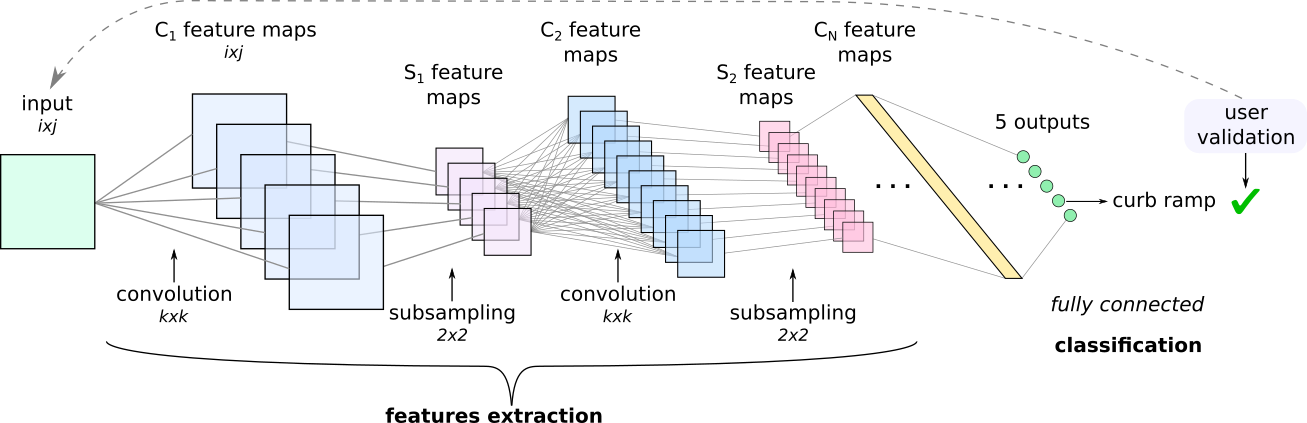
\includegraphics[width=1.0\linewidth]{architecture.png}
\end{center}
   \caption{A CNN detecting a curb ramp. User checking may disable the label associated with this image if the result is a false positive.}\label{cnn}
\end{figure}


E.g., if someone sees a curb ramp on a picture, he will be able to digitize it more accurately and marking it as a more or less friendly curb ramp (fig.\,\ref{curbramppicture}). An other example would let the user annotate a sidewalk surface width as %"not crossable for two wheelchairs" or 
"no possible way for a single wheelchair" based on the perceived width on the given picture. If depth information is also available for the given image, 
a tool \colorbox{green}{could you explain all the tools you have proposed ->	} may also be provided to directly measure distances onto the image.
\colorbox{yellow}{it is a methodology paper, the reader need to understand our methodology after read our paper}



\begin{figure}[ht]
\begin{center}
%\fbox{\rule{0pt}{2in} \rule{0.9\linewidth}{0pt}}
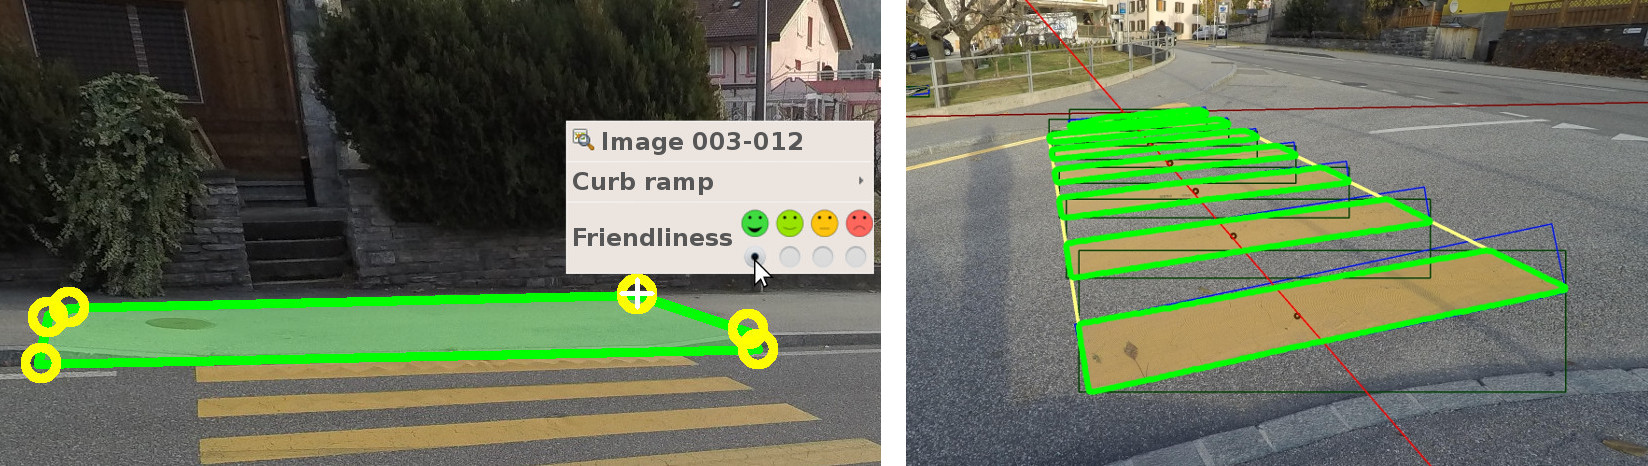
\includegraphics[width=1.0\linewidth]{curb_ramp_crosswalk01.jpg}
\end{center}
   \caption{Image examples of a manually digitized curb ramp with a friendliness score selection toolbox (left) and a true positive automatically detected crosswalk (right).}\label{curbramppicture}
\end{figure}


This stage will also give the user a tool to check the features that were detected by algorithms. This important step provides two advantages. It will first classify automatically detected features according to a standard confusion matrix. And then, machine learning detection algorithms could be refined with these new positive and negative labeled images. Training and testing results will be tracked to avoid overfitting in addition to some optimizations.


\iffalse
\begin{enumerate}\setlength\itemsep{-0.0em}
\item it will classify detected features according to a standard confusion matrix.

\iffalse
\vspace*{-0.0em}
\begin{table}[ht]
\caption{Confusion matrix}\label{confmat}
%\resizebox{0.5\textwidth}{!}{%
\setlength\tabcolsep{12pt}
\begin{tabular}{ l r c c }
%\toprule
\multicolumn{2}{ c }{} & \multicolumn{2}{ c }{{Detection} } \\
%\addlinespace
\cmidrule{3-4}
& & \makecell{{Positive}} & \makecell{{Negative}} \\
\cmidrule{3-4}
\multirow{2}{*}[0.2em]{\raisebox{4em}{\rotatebox[origin=c]{90}{Ground}~\rotatebox[origin=c]{90}{truth}}} & \makecell{Positive} & {True positive} & {False negative}  \\ 
 & \makecell{Negative} & False positive & True negative \\ 
\cmidrule{3-4}
%\bottomrule
\end{tabular}
%}
\end{table}	
\fi

\item machine learning detection algorithms could be trained again with these new positive and negative labeled images. Training results will be tracked to avoid overfitting in addition to some optimizations.
\end{enumerate}
\fi



%#####################################
\subsubsection*{4) End-user route choice \colorbox{green}{assessment} and update}
%#####################################
The final application \colorbox{green}{final step? Yes,also, as each step = a dedicated app as stated line 1-2of previous column.} will directly target the impaired pedestrian street users. It will propose the route with the best DPLoS value between two points based on the weighted sum of the DPLoS of each $n$ edges composing the route as define by eq.\,\ref{dplostot}.

\begin{equation}
\mathrm{DPLoS}_{\mathit{\,route}} = \frac{1}{n}\sum{\mathrm{DPLoS}_{\,\mathit{edge\ n}}}
\label{dplostot}
\end{equation}

\begin{figure}[ht]
\begin{center}
%\fbox{\rule{0pt}{2in} \rule{0.9\linewidth}{0pt}}
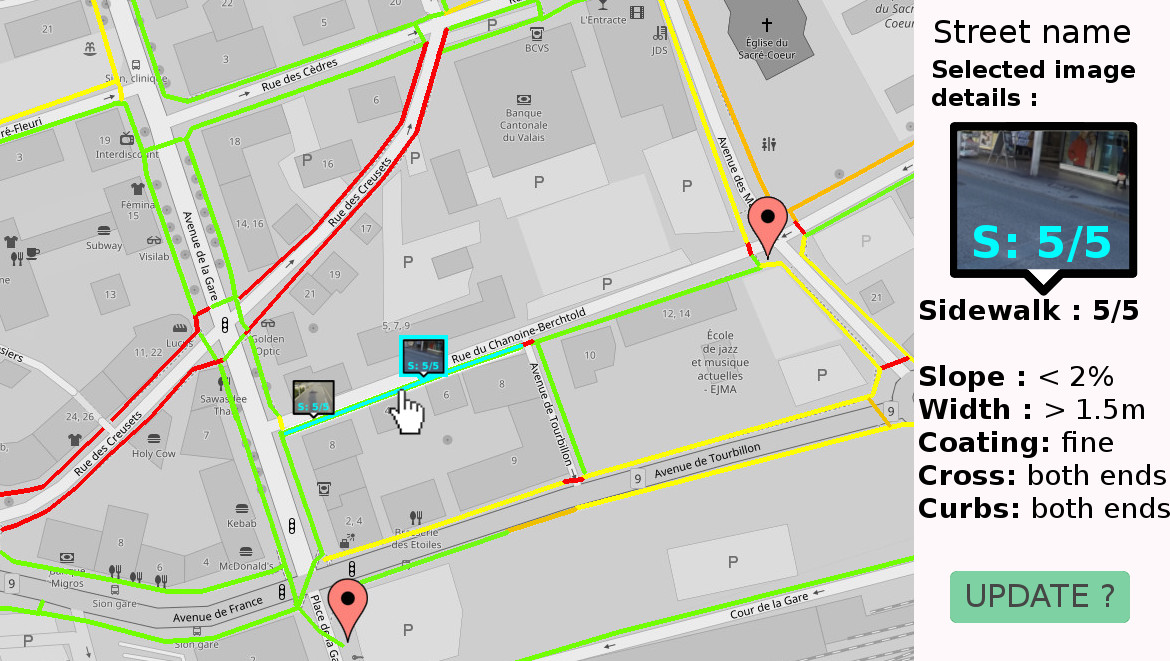
\includegraphics[width=1.0\linewidth]{example01.jpg}
\end{center}
   \caption{Prototype of the final application with edges of the pedestrian graph colored according to their DPLoS value (red=low value, green=high value). The selected edge shows that two different images participated to its score. Features' details for this edge and the selected image are shown on the right.}\label{finalapp}
\end{figure}



Informations about the edge as well as an update button (fig.\,\ref{finalapp}) will offer the user the possibility to give its feedback on a selected segment, for example if he sees an inadequate between the real world and a digitized feature. This will continuously improve the pedestrian network and update it as urban environment is changing.




%################################################################################
%\subsection{Computer Vision and Machine Learning}
%################################################################################




%################################################################################
%################################################################################
%\section{Preliminary Results and Evaluation}
%################################################################################
%################################################################################




%################################################################################
%################################################################################
\section{Conclusion and future work}
%################################################################################
%################################################################################
%This project is in its early stages. The first version of the DPLoS model is ready. The setting up of a database to store images metadata like geolocation, as well as algorithms and crowd-workers labeling results is taking place. This same database will serve the four different applications through APIs that need to be developed. It will finally need further investigating and tests regarding coupling of CV and ML algorithms. Database populating and labeling will be the most resource demanding tasks.


\colorbox{yellow}{proposition:}

In this paper, we describe how to build a crowdsourcing based disabled pedestrian level of service \colorbox{green}{routing} application using computer vision and machine learning. We analyze the existing technical algorithms for images processing, and explain their deficiencies. More importantly, we present the combination of these algorithms with crowdsourcing technologies to improve the \colorbox{green}{recall and the specificity} of \colorbox{green}{features} detection. Our methodology contains a four-step process, which gives a detailed view to the practitioners about this combination. The results highlight that the accuracy of the \colorbox{green}{features} detection \colorbox{yellow}{it will be... after many many tests} has been improved by apply the technology of crowdsourcing\colorbox{yellow}{crowdsourcing is not \emph{sensu stricto} a technology, isn't it?}. The next step for this study would be to implement our solution with the geolocation data from cities \colorbox{yellow}{I have carefully avoided speaking of the country in the paper}in Switzerland. The expected results will help people with mobility disabilities to plan their trips with an easy and secure way.

%################################################################################
%################################################################################
\section{Acknowledgement}
%################################################################################
%################################################################################
The Hasler Foundation supported the work described in this paper under grant number xxx. We thank ...


%%%%%%%%%%%%%%%%%%%%%%%%%%%%%%%%%%%%%%%%%%%%%%%%%%%%%%%%%%%%%%%%%%%%%%%%%%%%%%%%

\bibliographystyle{./myIEEEtran}
%\nocite{*} 
\bibliography{biblio}

\end{document}